\chapter{Conclusiones}

\section{Mejoras y ampliaciones}

Como se ha indicado en el apartado anterior el producto creado no es un juego finalizado si no un Mínimo producto viable (MVP). Es por el ello que aún hay trabajo por delante hasta que se convierta en un producto comercializable

Las siguientes son algunas de las posibles mejoras al sistema:

\begin{itemize}
	\item Implementar el sistema de guardado y cargado de partida.
	\item Incrementar la calidad/complejidad/cantidad de los diálogos.
	\item Utilizar modelos 3D propios.
	\item Aplicar animaciones a los modelos 3D
\end{itemize}

\section{Modelo de negocio}

Existen muchos métodos a la hora de comercializar un videojuego para plataformas móviles. En la actualidad las más usadas son la inclusión de publicidad, las compras dentro de la aplicación y la venta del videojuego en sí.
Se ha decidido tomar la última opción por los siguientes motivos: 

\begin{itemize}
	\item La inclusión de publicidad distrae la atención del jugador de lo que realmente importa: el juego. Además dependiendo de lo intrusiva que sea esta puede ser incluso molesta y entorpecer la experiencia de juego.
	\item Las compras dentro de la aplicación no se pueden llevar a cabo ya que tal cual ha sido diseñado el juego no hay elementos que se puedan comprar, ni con dinero real ni con dinero del juego.
\end{itemize}

De este modo se empleará un enfoque comercial en el que se venderá el videojuego y el usuario no tendrá que lidiar con publicidad o con contenido extra que se desbloquee pagando. Tendrá todo el potencial del juego en una única compra.

Debido a que el juego puede ser una herramienta muy útil en cursos de formación emprendedora se ofertará la compra de paquetes de licencias. De esta forma los organizadores del curso podrán comprar paquetes con licencias, que evidentemente serán mas baratas que licencias individuales, y repartirlas entre los asistentes al curso. 

También se pondrá a la venta en tiendas de aplicaciones como App store o Google Play para que cualquier persona, emprendedora o no,  interesada en el juego pueda comprarlo.

En la siguiente imagen (ver fig. \ref{leanCanvasDaVinci})  se muestra un Lienzo de modelo de negocio con una propuesta para la comercialización del producto.

\begin{figure}[H]
\begin{center}
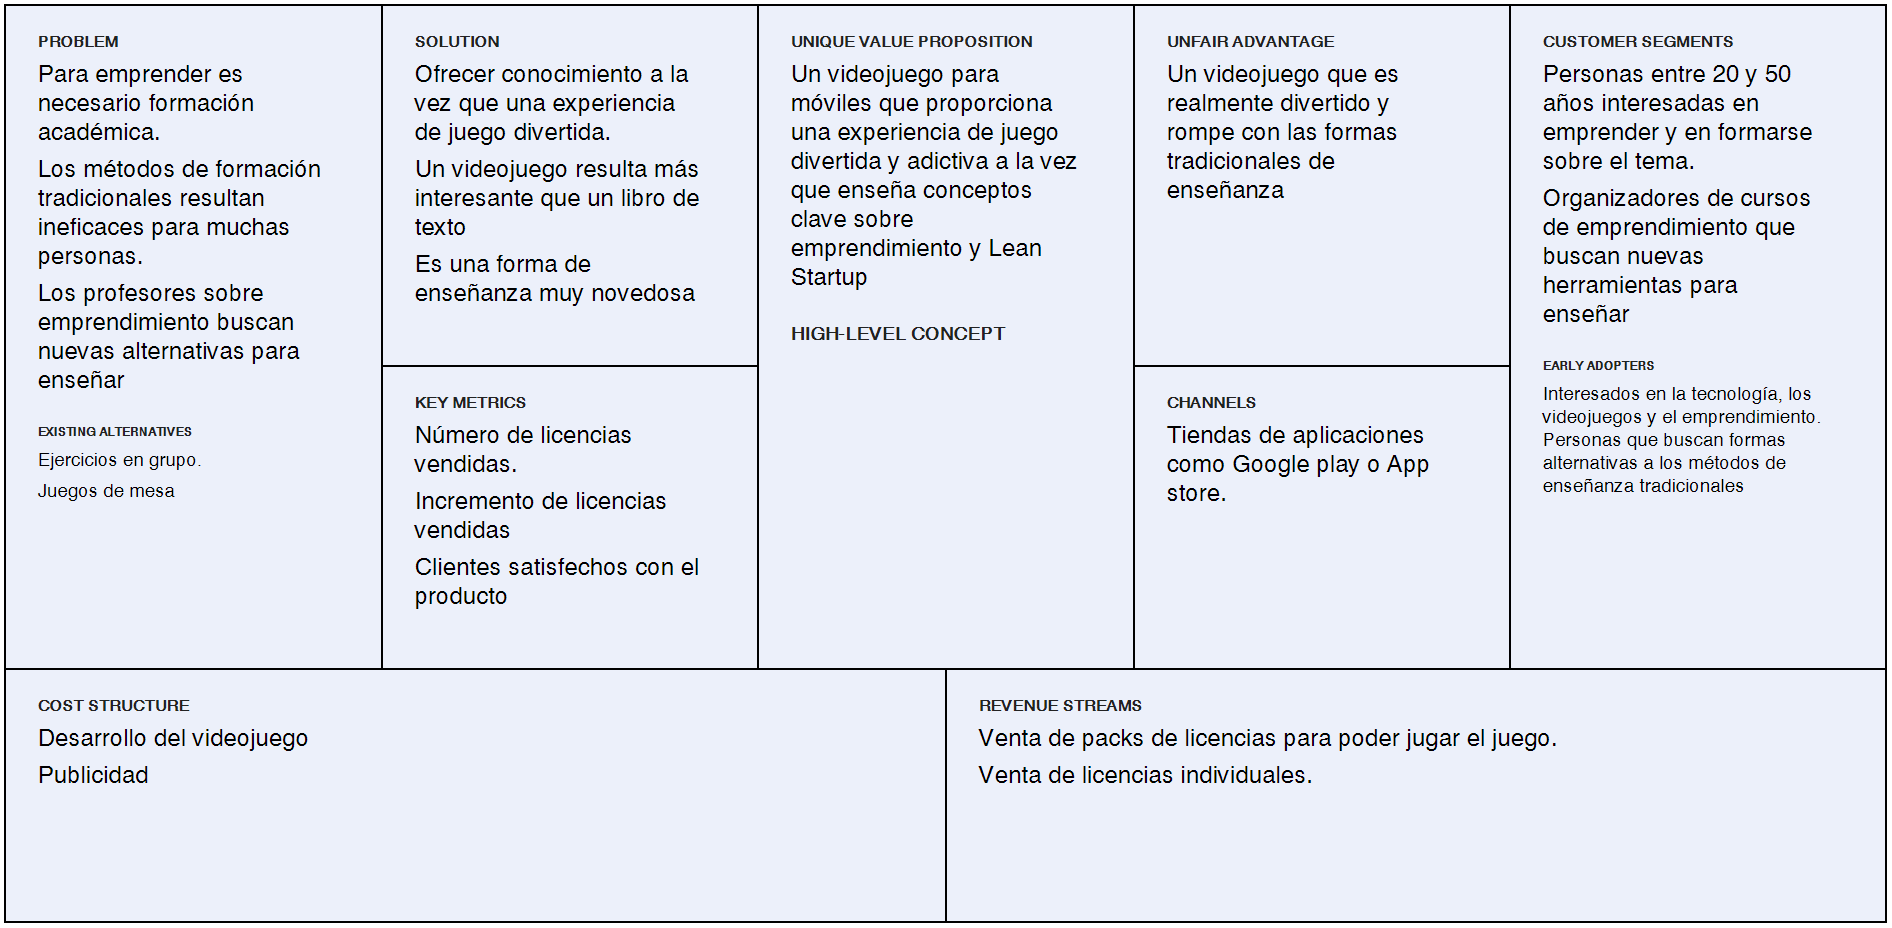
\includegraphics[scale=0.33]{imagenes/leanCanvasDaVinciStartup.png}
\caption{Lean canvas propuesto para este proyecto}
\label{leanCanvasDaVinci}
\end{center}
\end{figure}



